% ----------------------------------------------------
% Methodology
% ----------------------------------------------------
\documentclass[class=report,11pt,crop=false]{standalone}
% Page geometry
\usepackage[a4paper,margin=20mm,top=25mm,bottom=25mm]{geometry}
\usepackage{indentfirst}
% Font choice
\usepackage{lmodern}

% Use IEEE bibliography style
\bibliographystyle{IEEEtran}

% Line spacing
\usepackage{setspace}
\setstretch{1.20}

% Ensure UTF8 encoding
\usepackage[utf8]{inputenc}

% Language standard (not too important)
\usepackage[english]{babel}

% Skip a line in between paragraphs
\usepackage{parskip}

% For the creation of dummy text
\usepackage{blindtext}

% Math
\usepackage{amsmath}

\usepackage{enumitem}


% Header & Footer stuff
\usepackage{fancyhdr}
\pagestyle{fancy}
\fancyhead{}
\fancyhead[R]{\nouppercase{\rightmark}}
\fancyfoot{}
\fancyfoot[C]{\thepage}
\renewcommand{\headrulewidth}{0.0pt}
\renewcommand{\footrulewidth}{0.0pt}
\setlength{\headheight}{13.6pt}

% Epigraphs
\usepackage{epigraph}
\setlength\epigraphrule{0pt}
\setlength{\epigraphwidth}{0.65\textwidth}

% Colour
\usepackage{color}
\usepackage[usenames,dvipsnames]{xcolor}

% Hyperlinks & References
\usepackage{hyperref}
\definecolor{linkColour}{RGB}{77,71,200}%{0,144,208}%
\hypersetup{
    colorlinks=true,
    linkcolor=linkColour,
    filecolor=linkColour,
    urlcolor=linkColour,
    citecolor=linkColour,
}
\urlstyle{same}

% Automatically correct front-side quotes
\usepackage[autostyle=false, style=ukenglish]{csquotes}
\MakeOuterQuote{"}

% Graphics
\usepackage{graphicx}
\graphicspath{{Images/}{../Images/}}
\usepackage{makecell}
\usepackage{transparent}

% SI units
\usepackage{siunitx}

% Microtype goodness
\usepackage{microtype}

% Listings
\usepackage[T1]{fontenc}
\usepackage{listings}
\usepackage[scaled=0.8]{DejaVuSansMono}

% Custom colours for listings
\definecolor{backgroundColour}{RGB}{250,250,250}
\definecolor{commentColour}{RGB}{10, 204, 10}
\definecolor{identifierColour}{RGB}{0, 0, 255}%{196, 19, 66}
\definecolor{stringColour}{RGB}{255, 0, 255}
\definecolor{keywordColour}{RGB}{255,0,0}
\definecolor{lineNumbersColour}{RGB}{127,127,127}
\lstset{
  language=Python,
  captionpos=b,
  aboveskip=10pt,belowskip=10pt,
  backgroundcolor=\color{backgroundColour},
  basicstyle=\ttfamily,%\footnotesize,        % the size of the fonts that are used for the code
  breakatwhitespace=false,         % sets if automatic breaks should only happen at whitespace
  breaklines=true,                 % sets automatic line breaking
  postbreak=\mbox{\textcolor{red}{$\hookrightarrow$}\space},
  commentstyle=\color{commentColour},    % comment style
  identifierstyle=\color{identifierColour},
  stringstyle=\color{stringColour},
   keywordstyle=\color{keywordColour},       % keyword style
  %escapeinside={\%*}{*)},          % if you want to add LaTeX within your code
  extendedchars=true,              % lets you use non-ASCII characters; for 8-bits encodings only, does not work with UTF-8
  frame=single,	                   % adds a frame around the code
  keepspaces=true,                 % keeps spaces in text, useful for keeping indentation of code (possibly needs columns=flexible)
  morekeywords={*,...},            % if you want to add more keywords to the set
  numbers=left,                    % where to put the line-numbers; possible values are (none, left, right)
  numbersep=5pt,                   % how far the line-numbers are from the code
  numberstyle=\tiny\color{lineNumbersColour}, % the style that is used for the line-numbers
  rulecolor=\color{black},         % if not set, the frame-color may be changed on line-breaks within not-black text (e.g. comments (green here))
  showspaces=false,                % show spaces everywhere adding particular underscores; it overrides 'showstringspaces'
  showstringspaces=false,          % underline spaces within strings only
  showtabs=false,                  % show tabs within strings adding particular underscores
  stepnumber=1,                    % the step between two line-numbers. If it's 1, each line will be numbered
  tabsize=2,	                   % sets default tabsize to 2 spaces
  %title=\lstname                   % show the filename of files included with \lstinputlisting; also try caption instead of title
}

% Caption stuff
\usepackage[hypcap=true, justification=centering]{caption}
\usepackage{subcaption}

% Glossary package
% \usepackage[acronym]{glossaries}
\usepackage{glossaries-extra}
\setabbreviationstyle[acronym]{long-short}

% For Proofs & Theorems
\usepackage{amsthm}

% Maths symbols
\usepackage{amssymb}
\usepackage{mathrsfs}
\usepackage{mathtools}

% For algorithms
\usepackage[]{algorithm2e}

% Spacing stuff
\setlength{\abovecaptionskip}{5pt plus 3pt minus 2pt}
\setlength{\belowcaptionskip}{5pt plus 3pt minus 2pt}
\setlength{\textfloatsep}{10pt plus 3pt minus 2pt}
\setlength{\intextsep}{15pt plus 3pt minus 2pt}

% For aligning footnotes at bottom of page, instead of hugging text
\usepackage[bottom]{footmisc}

% Add LoF, Bib, etc. to ToC
\usepackage[nottoc]{tocbibind}

% SI
\usepackage{siunitx}

% For removing some whitespace in Chapter headings etc
\usepackage{etoolbox}
\makeatletter
\patchcmd{\@makechapterhead}{\vspace*{50\p@}}{\vspace*{-10pt}}{}{}%
\patchcmd{\@makeschapterhead}{\vspace*{50\p@}}{\vspace*{-10pt}}{}{}%
\makeatother
\makenoidxglossaries


\newacronym{fm}{FM}{Frequency Modulation}
\newacronym{am}{AM}{Amplitude Modulation}
\newacronym{em}{EM}{electromagnetic}
\newacronym{iq}{IQ}{In-phase and Quadrature}


\newacronym{dft}{DFT}{Discrete Fourier Transform}
\newacronym{idft}{IDFT}{Inverse Discrete Fourier Transform}
\newacronym{fft}{FFT}{Fast Fourier Transform}
\newacronym{ifft}{IFFT}{Inverse Fast Fourier Transform}

\newacronym{df}{DF}{Direction Finding}
\newacronym{rdf}{RDF}{Radio Direction Finding}
\newacronym{AoA}{AoA}{Angle of Arrival}
\newacronym{rf}{RF}{Radio Frequency}
\newacronym{sdr}{SDR}{Software-Defined Radio}
\newacronym{pd}{PD}{Phase-Difference}
\newacronym{vhf}{VHF}{Very High Frequency}
\newacronym{MHz}{MHz}{Megahertz}
\newacronym{db}{dB}{decibel}
\newacronym{dbm}{dBm}{Decibel-milliwatts}
\newacronym{rx}{Rx}{Receiver}
\newacronym{tx}{Tx}{Transmitter}
\newacronym{dsp}{DSP}{Digital Signal Processing}
\newacronym{vor}{VOR}{Very High Frequency Omnidirection Range}
\newacronym{gps}{GPS}{Global Position System}
\newacronym{adf}{ADF}{Automatic Direction Finders}
\newacronym{ndb}{NDB}{Non-Directional Beacon}
\newacronym{sm}{S meter}{Signal Strength Meter}
\newacronym{tdoa}{TDOA}{Time Difference of Arrival}
\newacronym{ham}{HAM}{an informal name for an amateur radio operator}
\newacronym{wbfm}{WBFM}{Wideband Frequency Modulation}
\newacronym{if}{IF}{Intermediate Frequency}
\newacronym{lp}{LP}{Low Pass}
\newacronym{API}{API}{Application Programming Interface}
\newacronym{fpga}{FPGA}{Field-Programmable Gate Array}
\newacronym{bw}{BW}{Bandwidth}
\newacronym{adc}{ADC}{Analog-to-digital converter}
\newacronym{tv}{Tv}{Television}
\newacronym{ai}{AI}{Artificial Intelligence}
\newacronym{lo}{LO}{Local Oscillator}
\newacronym{icasa}{ICASA}{Independent Communications Authority of South Africa}
\newacronym{usb}{USB}{Universal-serial Buss}
\newacronym{os}{OS}{Operating System}
\newacronym{mimo}{MIMO}{Mutliple input, Multiple output}
\newacronym{vna}{VNA}{Vector Network Analyser}
\newacronym{mse}{MSE}{Mean Squared Error}
\newacronym{SNR}{SNR}{Signal-to-Noise Ratio}

\begin{document}
\ifstandalone
\tableofcontents
\fi
% ----------------------------------------------------
\chapter{Direction Finding Methodology \label{ch:meth}}
\epigraph{``Imagination will often carry us to worlds that never were. But without it we go nowhere''
}%
    {\emph{---Carl Sagan}}
\vspace{0.5cm}
% ----------------------------------------------------

%---------------------------------
% Overview
%---------------------------------
\section{Overview}
This chapter aims to outline the process followed for the development of a \gls{sdr} \gls{df} system. To do so, first, the necessary signal processing theory is covered, with particular mention to the Frequency Domain, and subsequent Phase extraction methods and principles. Following on from the Literature discussed in Chapter \ref{ch:literature} surrounding \gls{sdr}, the hardware requirements for the system are analysed. The components needed for a \gls{rdf} system are presented, and the testing devices used. A software methodology follows, first discussing the requirements from the system, and the subsequent considerations and approaches to achieving this.
The penultimate section of this chapter deals with a suggested testing procedure for the project.

Note, however, this project is focused on \gls{rdf}, with the \emph{advantage} of \gls{sdr}. Thus, the focus of this chapter is to provide a logical approach to the engineering principles underpinning the project, and not a complete theoretical description and explanation of \gls{sdr} platforms. Additionally, while the fundamental signal processing theory is explained, it would not be practical to fully derive and explain what is in essence a complete field of electrical engineering. 


%---------------------------------
% Signal Theory
%---------------------------------
\section{Signal Theory \label{sec:Signal-Theory}}
The core basis of this project lies in the understanding and manipulation of signals in the frequency domain. In knowing that a \gls{sdr} produces data in \gls{iq} format (as explained in section \ref{sec:IQ}), this project aims to understand the workings with data of this nature.

\subsection{Frequency Domain}
The time and frequency domains are integral ideas in signal processing. In essence, they are alternative ways in which to represent the same signal, the Fourier transform is just a different representation of the same signal. As presented by Smith \cite{smith}, within the frequency domain, we are able to calculate the phase of a signal using less computational power. 
The Fourier Transform of $x(t)$ is defined as:
\begin{equation}
    X(\omega) = \int_{-\infty}^{\infty} x(t) e^{-j \omega t} \mathrm{dt}
\end{equation}
Noting Fourier transform pair above can be denoted as:
\begin{equation}
    x(t) \xleftrightarrow{\mathscr{F}} X(\omega)
\end{equation}
Importantly, we must understand that if a signal is modified in one domain, it will be changed in the other domain, although usually not in the same way \cite{sdr-for-engineers}. Therefore, when the incoming \gls{rf} signal is mixed (read multiplied in the time domain) with the \gls{lo}, we are performing convolution in the frequency domain. This is represented mathematically in table \ref{tab:fourier-pari}.

\begin{table}[h]
    \centering
    \begin{tabular}{c | c}
    \textbf{Time Signal} & \textbf{Fourier Transform Signal} \\
    \hline
    $x(t)h(t)$ & $ {\frac{1}{2 \pi}}  X(\omega) * H(\omega)$  
    \end{tabular}
    \caption{The Fourier transform pair for multiplication in the time domain}
    \label{tab:fourier-pari}
\end{table}

For application in this project, an understanding of the \gls{fft} and \gls{dft} is additionally necessary as these principles are used within \gls{pd} calculation. 

The \gls{dft} views both the time domain and the frequency domain signals as periodic. 
Signals acquired by a \gls{sdr} are stored into a buffer of N points (Figure \ref{fig:dft-time}). In this example, the 128 samples are produced by sampling an analogue signal at regular intervals. Thus sample 0 is distinct from sample 127, as they were acquired at different points in time. 

\begin{figure}[h]
    \centering
    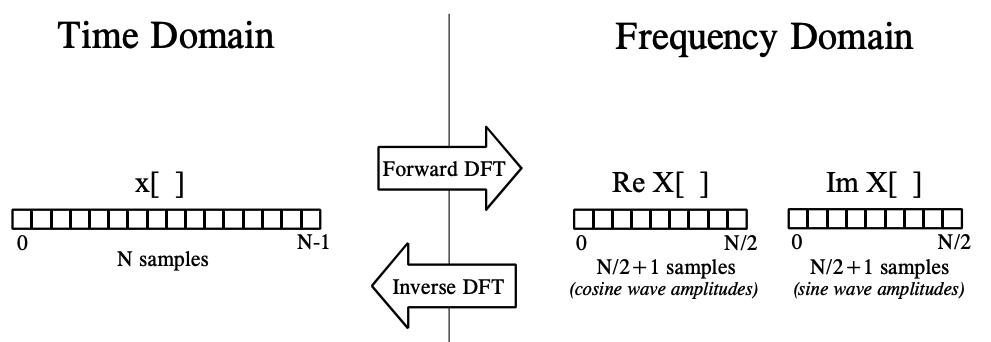
\includegraphics[width=0.8\textwidth]{Images/diagrams/DFT-time.png}
    \caption{Description of the Discrete Fourier Transform terminology. Represented by the time-domain buffer, x[ ] and frequency domain, which the DFT produces as two signals: ReX[ ] and ImX[ ]. \cite{engineers-dsp}}
    \label{fig:dft-time}
\end{figure}


However, since the \gls{dft} is periodic, the samples are viewed to be a single period of a signal with an infinitely long period. Figure \ref{fig:dft} represents this by showing the left side of the acquired signal connected to the right side of the duplicated signal. This can be thought of as wrapping.

\begin{figure}[h]
    \centering
    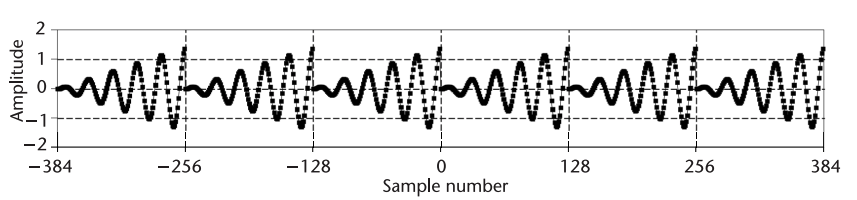
\includegraphics[width=0.8\textwidth]{Images/diagrams/dft.png}
    \caption{Periodicity of the DFT’s time-domain signal. The time-domain can be viewed as N
as an infinitely long periodic signal. \cite{engineers-dsp}}
    \label{fig:dft}
\end{figure}

It is for this reason that it is imperative to implement a windowing function before the application of the \gls{fft} of the captured signals. In doing so, the window function is multiplied by the captured signal and removes the discontinuities by forcing them to zero \cite{window}. This leaves only the desired portion of the signal to be processed by the \gls{fft}, and this portion is a complete cycle.

There are several ways to calculate the \gls{dft}: solving simultaneous linear equations, correlation, or the \gls{fft}. This method is incredibly efficient (reducing computation in the order of magnitudes), and while it is a complicated algorithm for \gls{dsp}, there exist many libraries (namely \emph{NumPy}) where the internal workings are left obscured, and given one input vector of samples, the .fft() function will produce one frequency domain version of the samples as a vector. The size of the output is always equal to that of the input. By increasing the number of samples in the input vector, the resolution obtained in the frequency domain will increase. 

\subsection{Sampling Rate}
An additional consideration for the project is that of the sampling rate and in turn the Nyquist Sampling theorem. The traditional Nyquist theorem states  that a real signal, $x(t)$, that is bandlimited to $B$Hz can be reconstructed without error if sampled at a rate $R$ where $R > 2B$ \cite{sdr-for-engineers}. This is called the minimum sampling frequency or Nyquist rate where $Fs = 2B$Hz.
\begin{figure}[h]
    \centering
    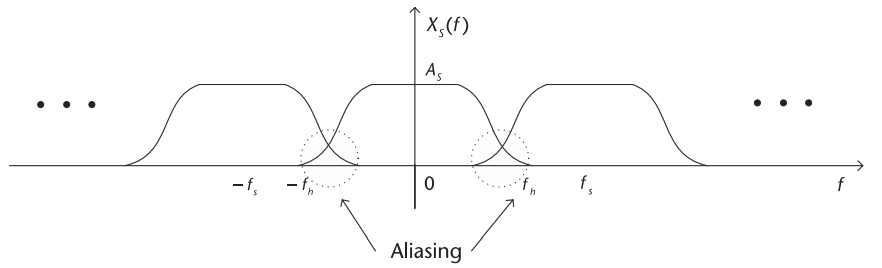
\includegraphics[width=0.8\textwidth]{Images/diagrams/aliasing.png}
    \caption{The spectrum of the digitally sampled signal x(t) where Fs < B resulting in aliasing from an unsatisfied Nyquist theorem \cite{sdr-for-engineers}}
    \label{fig:aliasing}
\end{figure}
    
To further extend the Nyquist theorem, Smith \cite{engineers-dsp} presents that sampling at a rate of $f_s$ and with only real samples, then one can unambiguously represent the content of a signal within the bound $[0, \frac{f_s}{2}) $  (although there is a caveat for bandpass sampling). Since the real signal exhibits conjugate symmetry in the frequency domain, no additional information can be held in the other half of the spectrum. 

Furthermore, with complex (\gls{iq}) signals sampled at $f_s$, the represented range is $-\frac{f_s}{2}$ to $\frac{f_s}{2}$. Meaning that by sampling at $f_s$ for complex signals, one can unambiguously represent the content of the signal. 

Noting at this stage that the frequency of the signal $f_s$ is the difference component of the $f_c \times f_{LO} $ \cite{superhet}. Suppose:
\begin{equation*}
    x(t) = A_1 \cos{(\omega_0 t + \phi(t))} 
\end{equation*}
\begin{equation*}
    LO(t) = A_2 \cos{(\omega_{LO} t)} 
\end{equation*}
Recalling the trigonometric identity:
\begin{equation}
    \cos(A + B) = \cos A \cos B - \sin A\sin B
\end{equation}

Applying this identity to $x(t) \times LO(t)$:

\begin{equation*}
\begin{split}
    & = \frac{A_1 A_2}{2} [\cos \phi (\cos(\omega_{LO} + \omega_0)t + (\cos(\omega_{LO} - \omega_0)t ] - [\sin \phi (\sin(\omega_{LO} + \omega_0)t + (\sin(\omega_{LO} - \omega_0)t ] \\
    & = \frac{A_1 A_2}{2} [\cos((\omega_{LO} + \omega_0)t + \phi(t)) + \cos((\omega_{LO} - \omega_0)t + \phi(t)]
\end{split}
\end{equation*}

\begin{figure}[h]
    \centering
    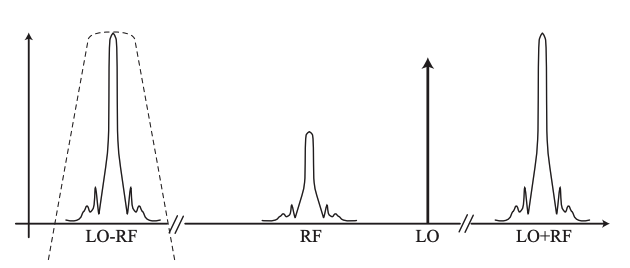
\includegraphics[width=0.8\textwidth]{Images/diagrams/LO_convolution.png}
    \caption{Multiplication of $f_c$ with the Local Oscillator leading to sum and difference components of the mixed RF signal.}
    \label{fig:LO}
\end{figure}

\subsection{Phase Measurement \label{phase-measurement}}
The basis of this project is to be able to extract the phase from a received \gls{rf} signal. 
This \gls{rf} wave is a type of \gls{em} radiation, and modulated to carry information (either by \gls{am} or \gls{fm}). The arrival of the wave-front can be assumed as a plane wave if the distance between the transmitter and the \gls{rx} antennas is significantly greater than the wavelength of the signal \cite{phase-diff-calc}. 

Remembering equation \ref{eq:IQ-general}, leading to equations \ref{eq:I} and \ref{eq:Q}, stated here for convenience:
\begin{equation}
    I = A_2 \sin(2 \pi f t) 
    \label{eq:I}
\end{equation}
\begin{equation}
    Q = A_2 \cos(2 \pi f t)
    \label{eq:Q}
\end{equation}
And referring back to figure \ref{fig:IQ}, from the complex number $I + j Q$, the magnitude and phase can be extracted:
\begin{equation}
    magnitude = \sqrt{I^2 + Q^2} 
\end{equation}
\begin{equation}
    phase = \arctan (\frac{Q}{I})
\end{equation}

Additionally, the application Eulers formula \cite{engineers-dsp} is useful for the \gls{AoA} calculation. 
\begin{equation}
    \begin{split}
        V(t) & = \cos{(\omega t)} \pm j \sin{(\omega t)} \\
        & = e^{ \pm j (\omega t)}
    \end{split}
\end{equation}

The data streamed out of a \gls{sdr} is stored into a binary file of type complex (32bit or 64bit depending on the host computer) \cite{gnuradio}, stored in the format $IQIQIQ$. After reading of the file, processing the vector array into real and imaginary components is trivial with a built-in \textsc{Python} package such as NumPy. Using NumPy one can use $np.abs(x)$ and $np.angle(x)$ for the magnitude and phase respectively. If the input is a complex number or an array of complex numbers and the output will be a real float number(s).

\subsection{Angle of Arrival}
To measure the radio wave, the frequency of said wave is observed, and from frequency, we can determine the wavelength from \cite{radio-waves}:
\begin{equation}
    \lambda = \frac{c}{f}
\end{equation}
Where $\lambda$ is the wavelength in meters, $c$ is the speed of light and $f$ is the frequency in Hertz. 

In order to calculate the \gls{AoA}, the \gls{pd} is needed. Section \ref{phase-measurement} dealt with the extract of the phase from an array. In order to calculate the \gls{pd}, one can simply take:
\begin{equation}
    \Delta \phi = \phi_2 - \phi_1
\end{equation}

In a system where there are two antenna, the \gls{AoA} can be calculated by (Figure \ref{fig:phase_interfer}) \cite{phase-diff-calc}:
\begin{equation}
    \theta = \arcsin(\frac{\lambda \Delta \phi}{2 \pi s} ) 
    \label{eq:pd-theta}
\end{equation}


An alternative method for \gls{AoA} calculation is presented in equation \ref{eq:conjugate}. The method relies on on the extraction of phase from a complex signal which can be represented by:
\begin{equation*}
    x(t) = A_1 e^{-j(\omega_0t + \phi)}
\end{equation*}
Multiplying a complex signal by the conjugate of the second complex signal allows for the extraction of the phase difference as seen in:
\begin{equation}
    x_1(t) \times (x_2(t)^*)
    \label{eq:conjugate}
\end{equation}

\begin{equation}
    \begin{split}
        \gls{AoA} & = angle(A_1 e^{j(\omega t + \phi_1)} * A_2e^{-j(\omega t + \phi_2)}) \\
        & = angle(A_1 * A_2  e^{j(\omega t + \phi_1 - \omega t - \phi_2)}) \\
        & = angle(A_1 * A_2  e^{j(\phi_1 - \phi_2)}) \\
        & = (\phi_1 - \phi_2)
\end{split}
\end{equation}

The ambiguity arises from an inability in which to resolve if the \gls{AoA} of the incident wavefront comes from in-front or behind-of the antenna array. It has previously been stated that equation \ref{eq:pd-theta} represents an angle between [$-\frac{pi}{2}, \frac{\pi}{2}$]. This is shown in figure \ref{fig:ambiguity}.

\begin{figure}[h]
    \centering
    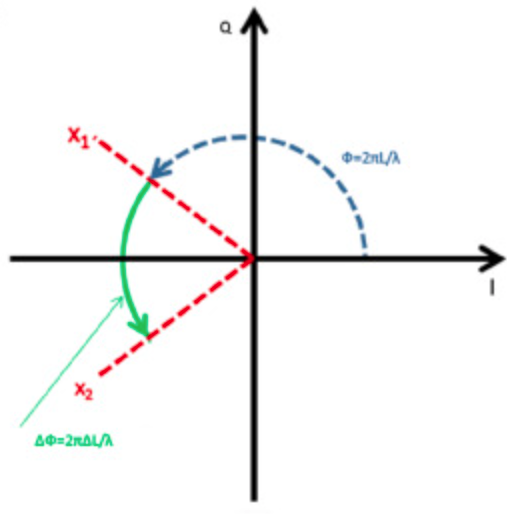
\includegraphics[width=0.4\textwidth]{Images/diagrams/ambiguity.png}
    \caption{Unresolved ambiguous AoA $x_1$ and $x_2$ polar coordinates from two antenna array example}
    \label{fig:ambiguity}
\end{figure}

This assumes the \gls{fft} has been already been performed. 


%---------------------------------
% Hardware
%---------------------------------
\section{Hardware}
For a working prototype to be developed for this project, much time was spent in understanding the different hardware components and making educated decisions for which devices would be most appropriate, based on research performed in chapter~\ref{ch:literature}. The following section details the approaches and considerations for each major hardware component for the \gls{rdf} system. 

\subsection{Host Computer}
The general-purpose computer for this project would perform two operations. Firstly, the computer would be used to interface, initialise and control the chosen \gls{sdr} through installed drivers. Secondly, data would be streamed from the \gls{sdr} to the computer, and perform all of the \gls{dsp} locally on the computer. In dealing with frequencies around the 150MHz band, the CPU would need to be able to handle the rate of processing required. Additionally, the host computer would need \gls{usb} 3.x ports for the data transfer rates of this project. 

At this point, it is important to note that the host computer will provide power to the \gls{sdr} device through the \gls{usb} ports. \gls{usb}2.x provides a maximum current of 500mA, which in some cases may be underpowered for the \gls{sdr} device. On the other hand, \gls{usb}3.x has a maximum current output of 900mA, which is sufficient to power the \gls{sdr} device. 

\subsubsection{Driver}
For a project of this nature, the most important consideration for the host computer was that of driver availability. Significant time was spent installing, re-installing, researching and anguishing over drivers to control the \gls{sdr}. 

For practical purposes, the driver is the abstraction layer for the \gls{sdr}. The driver allows communication from the system designer as a high-level instruction set to be translated to low-level register control instructions. This is most commonly in the form of a bitstream, used to configure the \gls{fpga}. Additional control of the sampling rate and channel ports for \gls{rx} were configured in this manner. 

The final purpose of the drivers was to control the data transfer link between the host computer and the \gls{sdr} internal memory. The ability to control the internal buffers and their manner of operation were considered. 

Based on similar projects to this work (see \cite{sdr-modern-approach}, \cite{pd-thesis}, \cite{gnu-con17}, \cite{kerberos} and \cite{myriad}) all suggested the use of a Linux based operating system for the availability of drivers, support and control over packages and the \gls{os}. For this project, the Raspberry Pi 4 Model B is used.  


\subsection{Software Defined Radio\label{sec:IQ}}
Paramount to the success of this project, and the most important hardware consideration is the \gls{sdr} platform. Interfacing with the \gls{sdr} is controlled by the previously discussed Host computer, driver and software (to be discussed in the next section). However, the hardware components of the \gls{sdr} device need to be considered for the operation of the device. Additionally, for use in the project, the device must have both open-source software and hardware schematics.

\subsubsection{Local Oscillator}
The requirement for this project was a sampling of \gls{rf} of bands between 148MHz to 152MHz, the common wildlife telemetry bands allocated by \gls{icasa} \cite{wild-life-telem}. The \gls{lo} is used to produce the \gls{iq} sampled data, and in \gls{vhf} ranges, using the different components of the mixed-signal needs to be of high enough frequency to allow sampling to accurately capture the signal according to Nyquist \cite{engineers-dsp}. Thus any \gls{sdr} with a good quality \gls{lo} of $>30$MHz would be considered, noting this must then be in line with the maximum sampling rate of the device. 

\subsubsection{Synchronisation of channels}
For Phase interferometry, when comparing two \gls{rx} signals, the signals must be both time-aligned signals and sampled synchronously. 
While Section \ref{sec:Design/HardwareDesign} deals further with the device selection, at this point it is worth noting that the device chosen had 2X2 \gls{mimo} integration in the \gls{fpga}, allowing for the connection of two \gls{rx} channels without additional hardware, and more impactful for this project, the default synchronisation of two channels. 

\subsubsection{Frequency range}
The frequency range of operation has been mentioned numerous times, and the \gls{sdr} device selected would need to be capable of \gls{rx} on two channels, and thus two \gls{adc} at this frequency range for it to be suitable for the project. 

\subsubsection{Transfer speed}
To transfer the sampled data, \gls{usb}3.0 is the only option considered. The rate of transfer will depend on the length of the signal capture, and the timing of the loop for calculations. \gls{usb}3.0 is the only available technology capable of handling the constraints of this project, even if the tuning and optimisation transfer were not considered. With limited time and project budget, this project erred on the side of caution, and simply did not consider any other technologies. 

\subsubsection{Bandwidth}
While bandwidth can be a function of frequency depending on the \gls{sdr} \cite{sdr-for-engineers}, a minimum bandwidth of 2MHz would be needed to cover the entire frequency range of interest. While for testing purposes this was not necessary, for the desired application of this project the consideration needs to be accounted for. 

\subsubsection{\gls{fpga}}
The use of \gls{fpga} is the most common processor in modern \gls{sdr}. The choice of such hardware is not considered in this project, as it is generally understood that if the above-mentioned requirements are met, then the \gls{fpga} would be capable of processing and performing this. More time understanding the internal workings of the \gls{fpga} would have been beneficial and to future work on this project.

\subsubsection{\gls{adc}}
The sampling of each antenna must be both synchronised and time-aligned. With data at each antenna being sampled as \gls{iq} channels, this means a minimum of four (4) \gls{adc} must be integrated in the \gls{sdr} architecture. The quantisation of this is also considered, and generally, most \gls{sdr} devices implement a 12-bit \gls{adc}. While \gls{tx} will not be used for this project, traditionally a true single-chip (2x) \gls{mimo} device would be suggested. 


\subsubsection{IQ Data}
How a \gls{sdr} produces \gls{iq} data has previously been discussed. Yet, the processing of this data until now has not. Figure \ref{fig:IQ-sdr} provides a graphical view of the outputted data streams, which is streamed to the host computer. Further mention of the combination of the data streams is made in \ref{sec:Design/Software}, but as this project was limited in scope, delving into the transfer protocol, delays and scheduler were not achievable.

\begin{figure}[h]
    \centering
    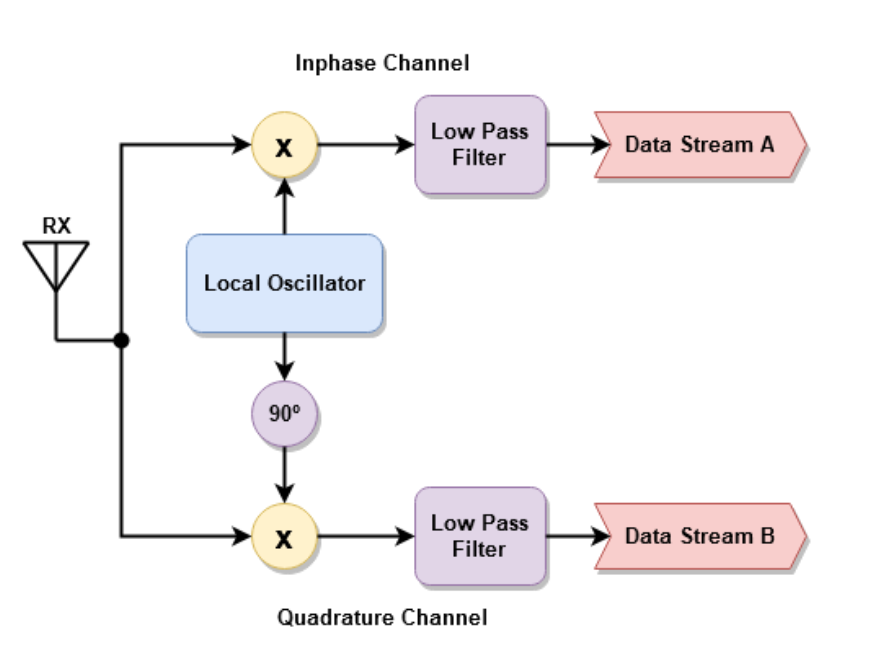
\includegraphics[width=0.6\textwidth]{Images/diagrams/IQ_data_SDR.png}
    \caption{A lock diagram of the general IQ operation in a SDR, with input antenna and resulting data streams.}
    \label{fig:IQ-sdr}
\end{figure}

Considering the above factors influencing the decision of which \gls{sdr} device to use in the project, the LimeSDR device was selected. In Chapter \ref{ch:design}, a detailed explanation of the features of the device will be given, system parameters discussed and detailed diagrams provided. This device was successful for the project and proved to be capable, but mention must be given to the KerberosSDR, which would have been more ideally suited, and prevented considerable headaches during the development of the project. Nevertheless, the LimeSDR was selected due to its availability within the University, and based off budget and time constraints for the project, suitable. The built-in \gls{mimo} and channel synchronisation were key in preventing further development into the correlation of signals in software processing. 

\begin{figure}[h]
    \centering
    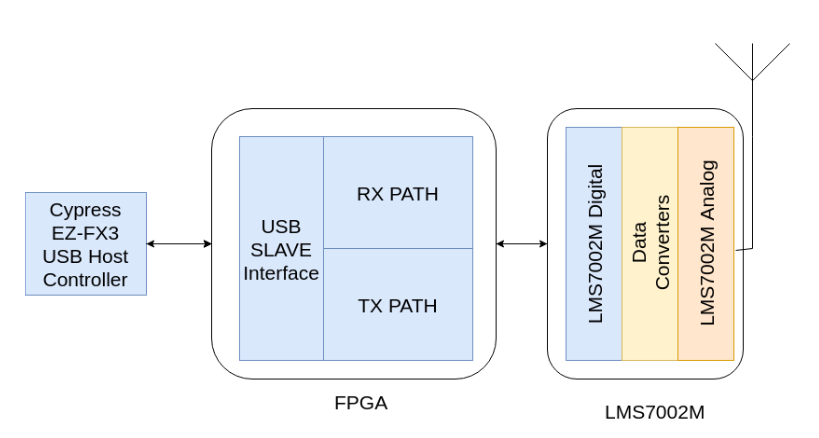
\includegraphics[width=0.8\textwidth]{Images/diagrams/LimeSDR-interface.png}
    \caption{Hardware controllers for the LimeSDR}
    \label{fig:limeSDR-hardware}
\end{figure}
\subsection{Antennas}
While antenna design falls outside the scope of this project, choosing a suitable antenna from both \gls{rx} channels as well as from \gls{tx} during testing was necessary. Without delving into the theory of antenna propagation patterns, resonance and reflection coefficients, a brief mention of the selection procedure will be made.

Firstly, this project needed two antennae for reception (\gls{rx}), one for transmission during testing (\gls{tx}), and should be matched to the frequency. 

Based off the frequency range of this project, connection to the correct \gls{rx} port for the LimeSDR will be discussed in chapter \ref{ch:design}, noting here that SMA connectors and coaxial cable RG58A/U were used. This was primarily due to its availability, however, taking into consideration table \ref{tab:coax} better selection can be considered in the future. Although out of scope of this project, mention of the considerations has been raised.

\begin{table}[h]
    \centering
    \begin{tabular}{c|c}
        Frequency (MHz)  & Attenuation (dB/100m)  \\
        \hline
        50 & 12.2\\
        100 & 17.8\\
        200 & 26.6\\
    \end{tabular}
    \caption{coaxial cable RG58A/U attenuation in decibels per 100m of cable}
    \label{tab:coax}
\end{table}

In understanding antenna resonance, thinking of an antenna as a tuned circuit that consists of inductance and capacitance makes sense. The resonance of the antenna is the frequency where the inductive and capacitive elements cancel each other out \cite{antenna}. This is then the frequency that the antenna is matched for, and will operate successfully at. Figure \ref{fig:antenna_resonance} describes this.

\begin{figure}[h]
    \centering
    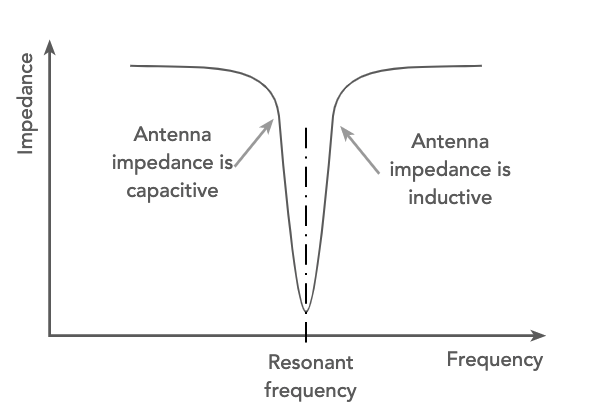
\includegraphics[width=0.5\textwidth]{Images/diagrams/antenna_resonance.png}
    \caption{The resonance frequency of an antenna is described as a variation of impedance.}
    \label{fig:antenna_resonance}
\end{figure}

To measure the resonance frequency of an antenna, a \gls{vna} is used. The \gls{vna} typically plots the parameter S11, which is a measure of power reflected from the antenna. The ratio of power outputted to the antenna, versus how much is then reflected back to the \gls{vna} is known as the reflection coefficient \cite{antenna}. Since antennas are designed to be low loss, we can assume the majority of the power outputted is radiated from the antenna. 
The theory of antenna follows then that if the antenna is well-matched for transmission, it will also be well matched for reception \cite{antenna}. 

The antennas used for this project was roughly $\frac{1}{4}$ wavelength monopole antenna, mounted to a ground plane as suggested by Marconi \cite{radio-history}.


\subsection{Testing Devices}
To generate a \gls{tx} signal used for testing, a signal generator accessible in the Microwave Lab at the University of Cape Town was used (Figure \ref{fig:function-gen}). This device was capable of producing a pure sin wave at 150.5MHz, the desired test frequency, and with control over the amplitude and output power, was well suited to the application.

\begin{figure}[h]
    \centering
    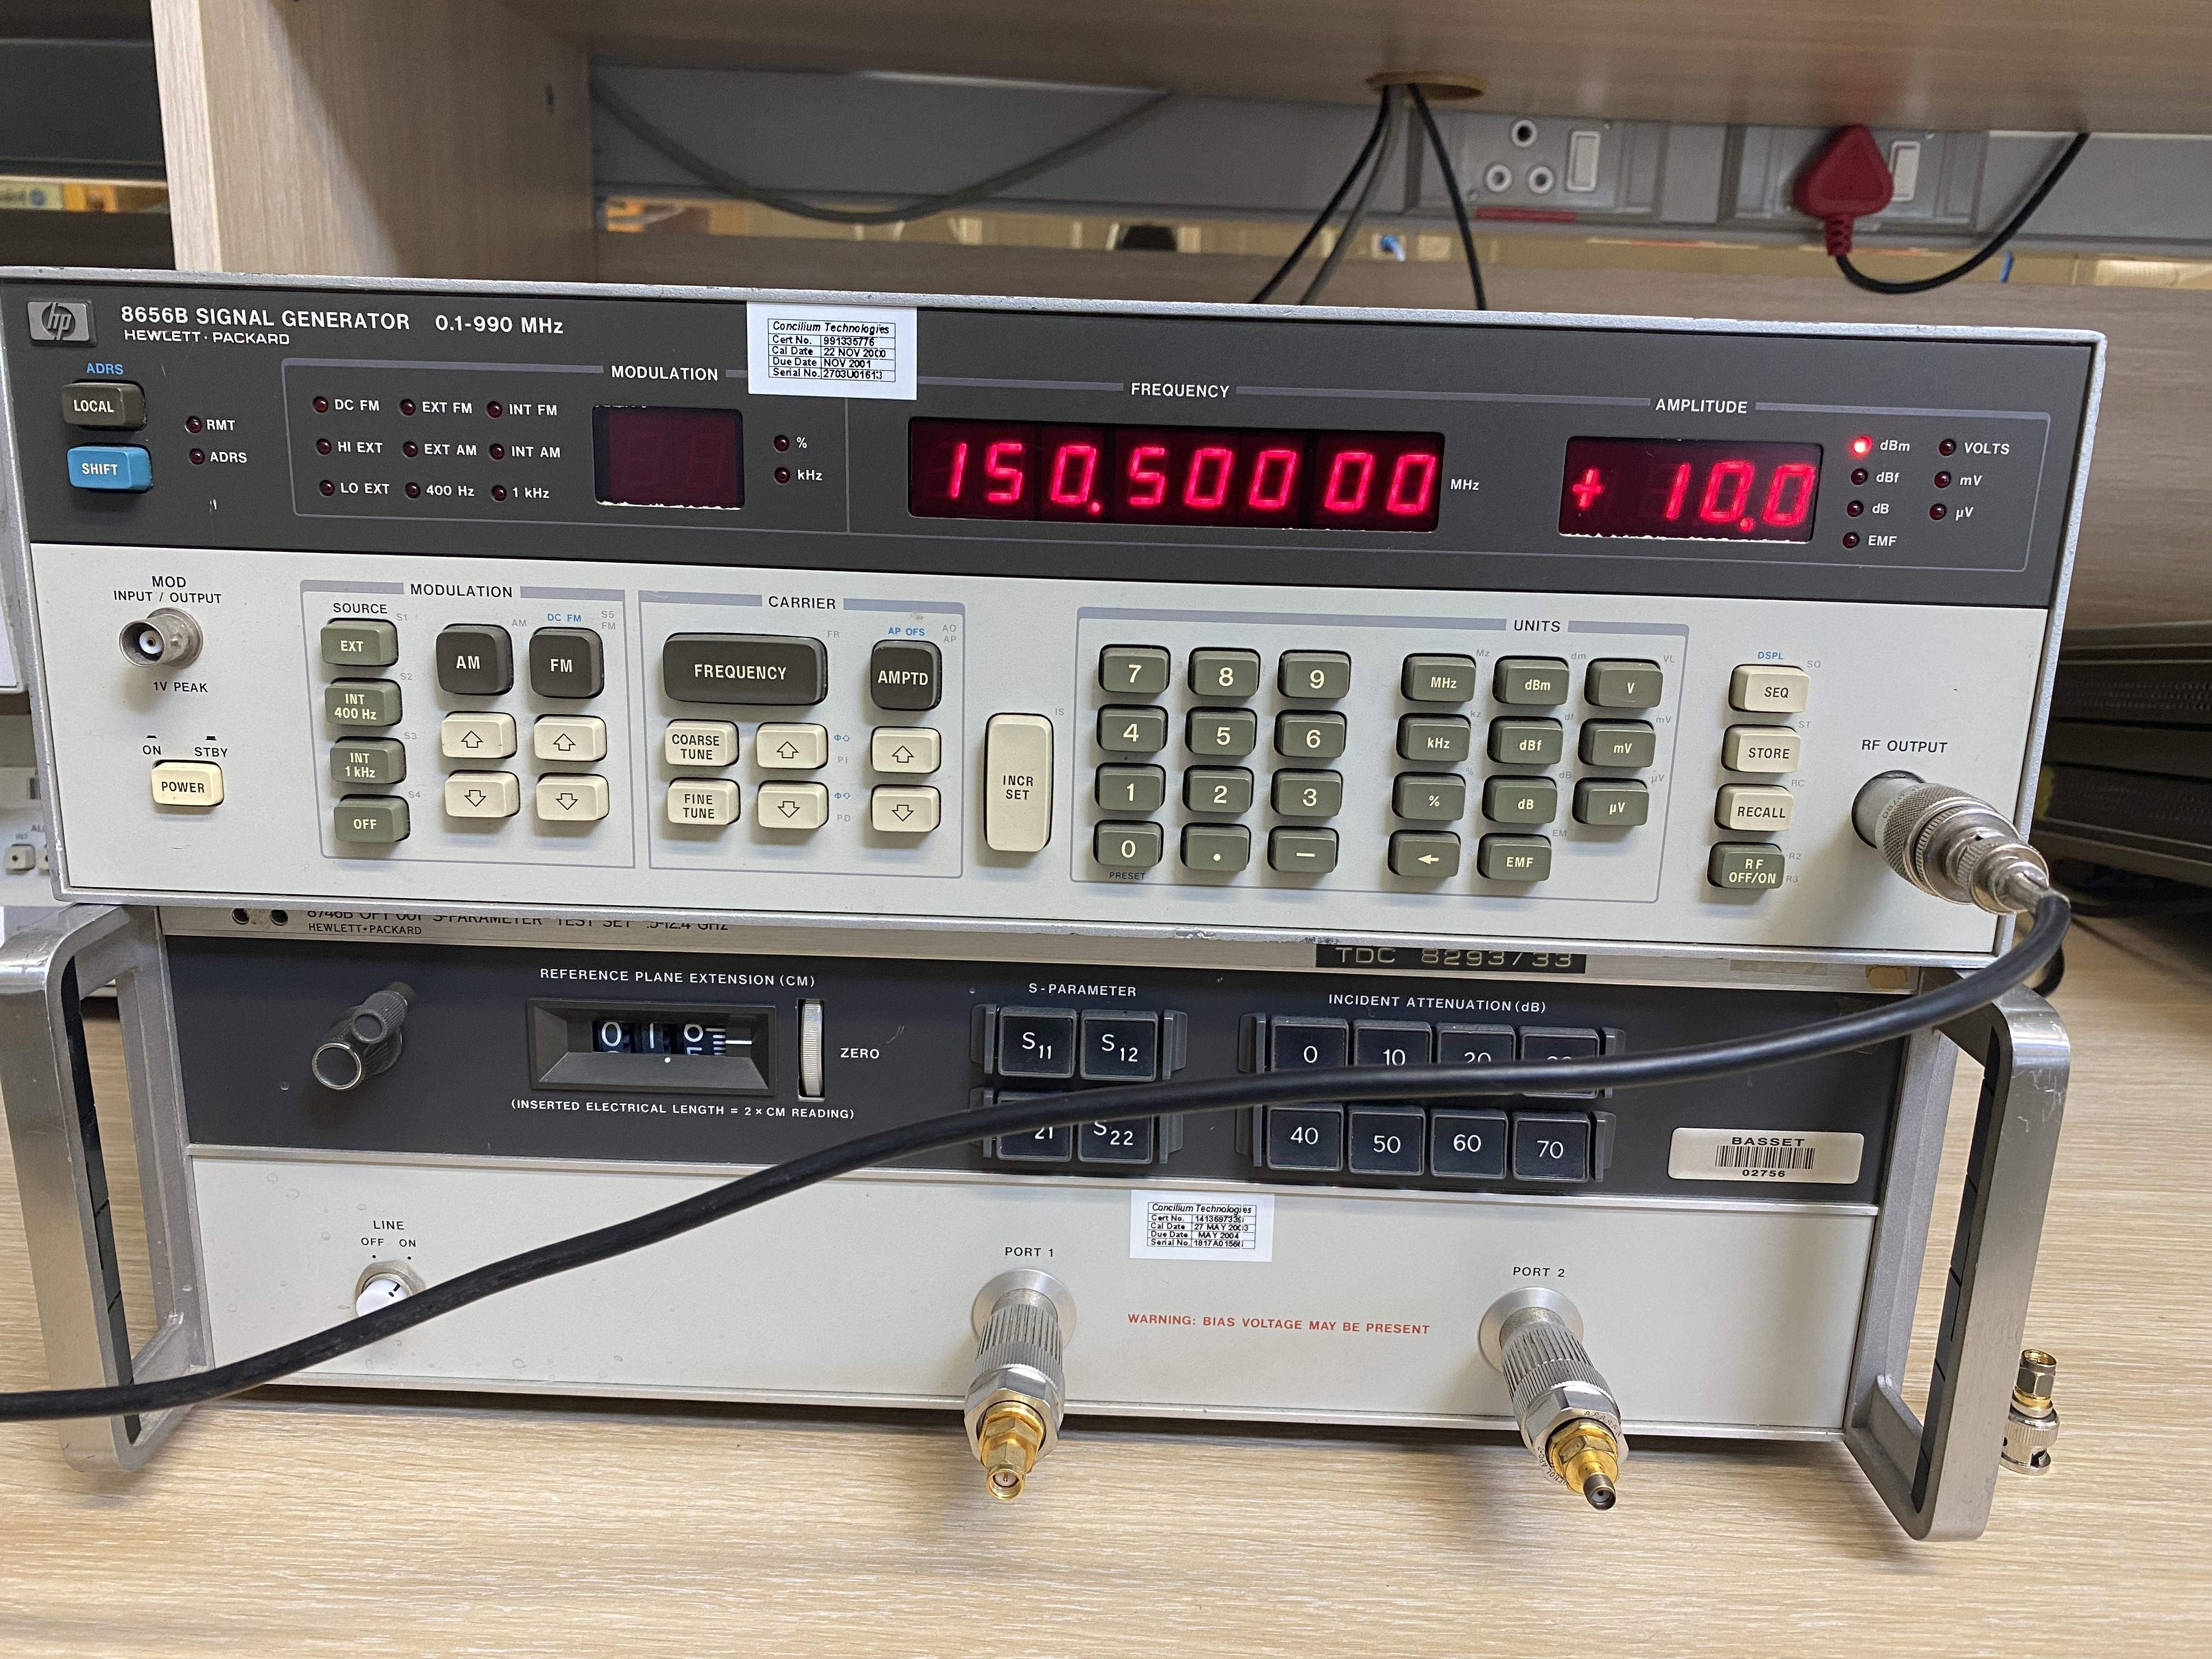
\includegraphics[width=0.6\textwidth]{Images/diagrams/signal_gen.jpg}
    \caption{A signal generator is used for testing, ensuring a pure sin wave of 150.5MHz is radiated with ample power for efficient testing.}
    \label{fig:function-gen}
\end{figure}
While this does not provide a real-world scenario for wildlife telemetry, the objective of the project was to prove that through difference in the phase measured at each antenna, the \gls{AoA} could be calculated and therefore \gls{rdf} was possible with an \gls{sdr}.

Additional testing for verification was performed on 89MHz, which in Cape Town is the radio station 5FM, to validate the \gls{sdr} device was working as expected.

%---------------------------------
% Software
%---------------------------------
\section{Software \label{sec:Software-Meth}}
The software used to control the \gls{sdr} device, and \textsc{Python} scripts used for both testing and data collection is depicted in Figure \ref{fig:uml}.

\begin{figure}[h]
    \centering
    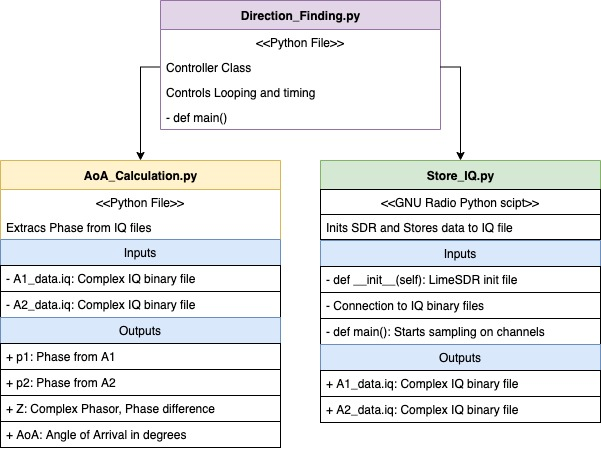
\includegraphics[width=0.8\textwidth]{Images/diagrams/class Software SDR.jpg}
    \caption{UML Class diagram to describe the project code structure.}
    \label{fig:uml}
\end{figure}
To understand the basic methodology of the processes needed to perform the testing and validation of this project the flow graph, Figure \ref{fig:flow} represents this. 

\begin{figure}[h]
    \centering
    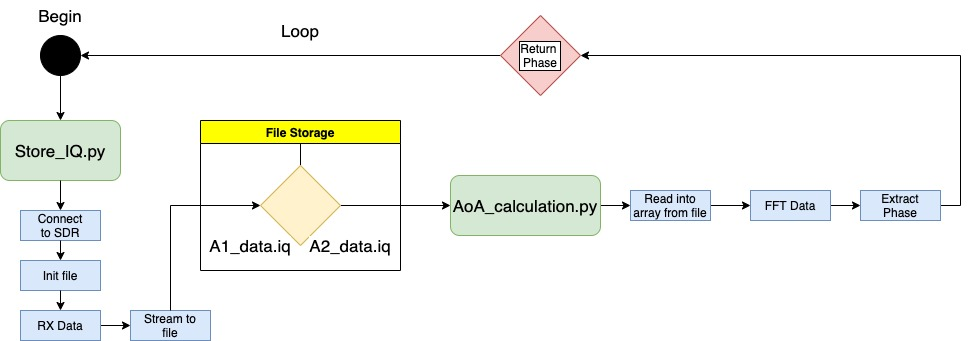
\includegraphics[width=0.8\textwidth]{Images/diagrams/Activity Software SDR.jpg}
    \caption{Flow graph for the processes executed by Python code from the project}
    \label{fig:flow}
\end{figure}


\subsection{Software Defined Radio Initialisation}
The initialisation of the \gls{sdr} device is performed using a bitstream file \footnote{register configuration files}, and sets the registers and ports on the \gls{fpga} and default behaviour of the device. In the context of this project, the LimeSuiteGUI open-source software is used to execute the \gls{API} function calls necessary, which can then be saved to an init file. 

First, the connection is made to the board, then the desired \gls{API} function calls run. Following this, the file is then saved for use by GNU Radio when connecting to the device during use. 

\begin{figure}[h]\centering
    \subfloat[Connection to device, based of serial number]{\label{a}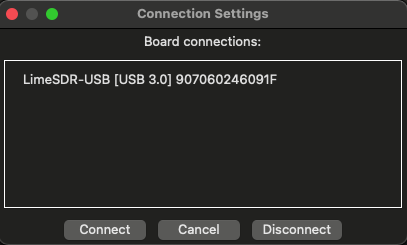
\includegraphics[width=.4\linewidth]{Images/diagrams/lime-connect.png}}\hspace{.5cm}
    \subfloat[Available \gls{API} functions]{\label{b}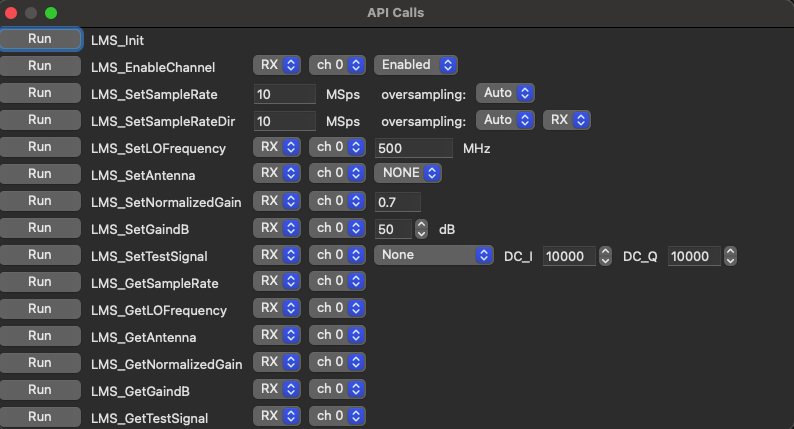
\includegraphics[width=.4\linewidth]{Images/diagrams/lime-api.png}}\hfill 
    \caption{LimeSuitGUI process for connecting to the SDR and generating a init file}
    \label{fig:phase-change}
\end{figure}

\subsection{GNU-Radio}
For this project, GNU Radio is used to interface with the \gls{sdr} device, control gain and antenna settings, sample data and stream samples to a binary file. The benefits of GNU Radio are described in Chapter \ref{ch:literature}, and project \cite{gnu-con17}. In order to use GNU Radio, the SoapySDR \gls{API} is implemented as described in Figure \ref{fig:limeSDR-interfacing-soapy}.

GNU Radio is based off of \textsc{Python}, making development easy to connect blocks and create flow graphs. The blocks themselves are written in \textsc{C++}, and can be edited for finer control if needed. With GNU Radio, one is able to write applications that are capable of receiving real-time data, process this data, and outputting to digital streams \cite{gnuradio}. 

GNU Radio is specifically designed to handle the streaming of large amounts of data in real-time between parallel computational nodes \cite{gnu-delays}. The flow of data between the source and the sink is described in a flow graph and controlled by the GNU Radio scheduler.

\begin{figure}
    \centering
    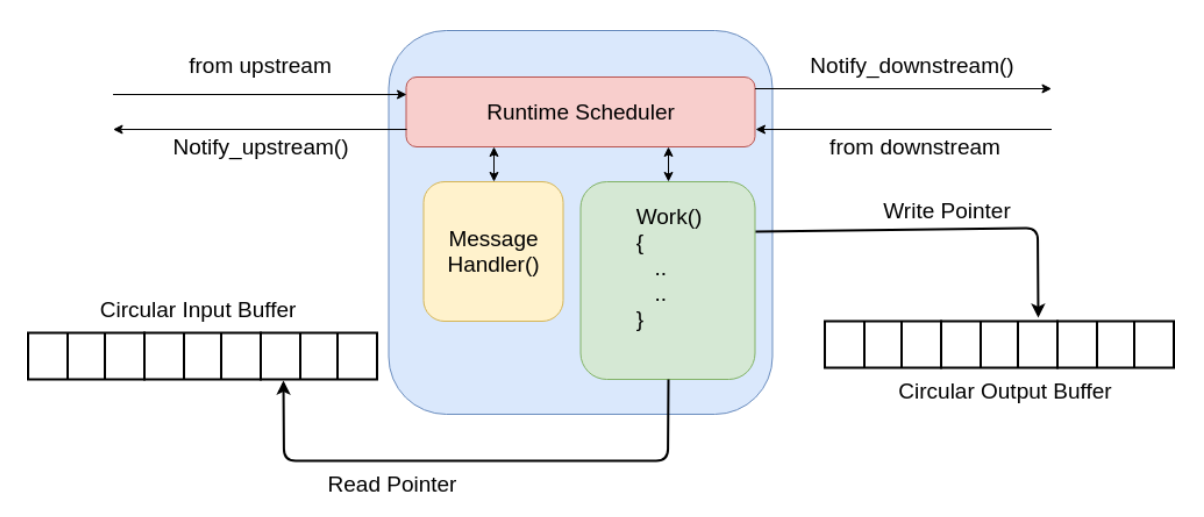
\includegraphics[width=0.8\textwidth]{Images/diagrams/gnu-scheduler.png}
    \caption{The architecture of the GNU Radio scheduler and runtime blocks}
    \label{fig:gnu-scheduler}
\end{figure}

\subsection{Synchronisation}
This key aspect of the software is critical to the workings of the project. The \gls{sdr} device selected has built-in \gls{mimo} and default synchronisation, however, this does not ensure that the samples are time-aligned. The scope of the project prevented a deep-dive into the internal delays, the scheduler of both the \gls{sdr} and the host computer, and function calls, however as it was critical to the workings of the project, a validation test was performed to ensure correctness. 

The advantage of GNU Radio as the software of choice for this project was the scheduler it uses (as depicted in figure \ref{fig:gnu-scheduler}). Much research has been done into the timing characteristics of the scheduler by Harza, see \cite{gnu-delays}. The information following is based of the Masters Thesis produced.

The scheduler controls the flow graph developed and allocates the buffers and initialises threads for each block. When the flow graph is run, the scheduler performs memory management and alignment of the data in each buffer \cite{gnu-delays}. Following alignment, the scheduler passes points to the \emph{work} function and executes one cycle of the \emph{main} function. Post this, the scheduler returns information and updates the state of blocks. 

\subsection{DC Offset}
The drawback of mixing a signal with a \gls{lo}, is the induced DC component that will now occur at the centre frequency as a result of the \gls{lo} \cite{sdr-for-engineers}. While the \gls{sdr} device attempts to remove this by first viewing the received signals in the frequency domain without an incoming source, and then removing the spike, this is often not successful \cite{sdr-for-engineers}. 

An attempt to remove this offset can be made by taking the average of an entire complex array, and removing this value from each element within the array as follows:
\begin{lstlisting}[language=Python, caption=Python code to remove DC value from LO, label={lst-dc}]
import numpy as np

mean1 = np.mean(a1_data)
mean2 = np.mean(a2_data)

a1_dc = a1_data - mean1
a2_dc = a2_data - mean2 
\end{lstlisting}

%---------------------------------
% Testing Procedure
%---------------------------------
\section{Testing Procedure}
With the aim of this project being "to prove that through calculating the Phase Difference in received signals from two antennae, with the use of a \gls{sdr}, \gls{rdf} is possible", the following testing procedure was developed to allow for signal acquisition, validation and experimental data capture. 
The design and results for the following tests will be discussed in Chapters \ref{ch:design} and \ref{ch:results} respectively.

\subsection{FM Radio Stations}
The first test developed was for validation purposes, and not altogether related to the aim of this project. In order to ensure that the \gls{sdr} device was receiving data correctly, and subsequently storing data in a usable format, testing on 89MHz was conducted. 89MHz is the \gls{fm} radio station 5FM in Cape Town. 

Using the open-source software CubicSDR, the first objective was to initialise the \gls{sdr}, set the operating parameters to logical values, and receive signal data. This ensured the drivers installed were operational, and the \gls{API} was interfaced with the device. Applying a \gls{fm} demodulator, and passing the output to an audio sink, allowed for the demodulation and therefore listening to live radio. This test was conducted in order to validate two major factors: firstly, that the antenna was operating as expected, and secondly that the \gls{sdr} itself was capturing data on the desired frequency with the correct amplifier and gain settings. Figure \ref{fig:cubic-demod} shows a typical \gls{fm} demodulator for radio on a \gls{sdr} device. 

\begin{figure}[h!]
    \centering
    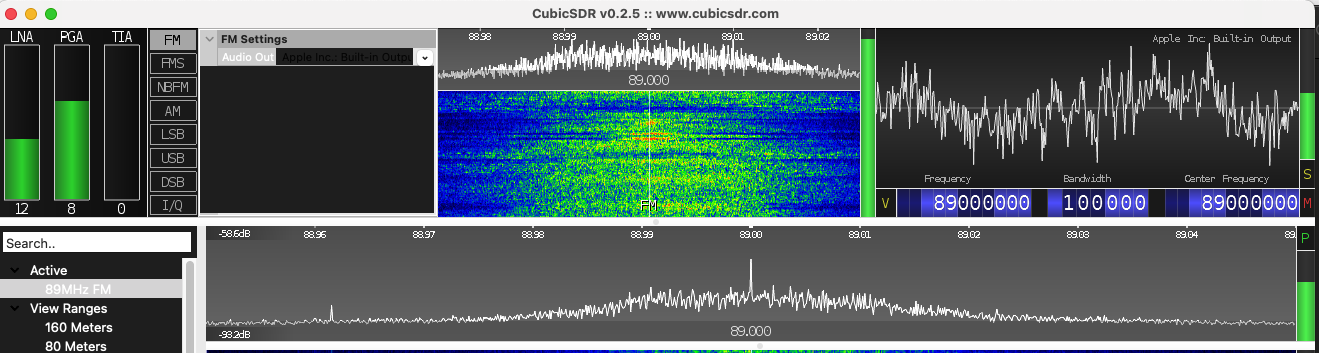
\includegraphics[width=0.95\textwidth]{Images/diagrams/fm_demod_cubicSDR.png}
    \caption{FM demodulator working on 89MHz using CubicSDR for testing of the device}
    \label{fig:cubic-demod}
\end{figure}

\subsection{Time Domain}
The next test performed for this project is to validate that the \gls{sdr} device is sampling the signals at both \gls{rx} antenna synchronously. This means that the signals would be both time-aligned, and sampled coherently. For the purposes of this project, ensuring the signals are time aligned is paramount to the correct \gls{pd} calculation. 

While the \gls{sdr} device uses a common clock as a reference for sampling of the \gls{adc}, this does not guarantee that the signals will be time-aligned, but rather that the signal sampling will be at fixed time offsets. The \gls{sdr} device chosen is claimed to be \gls{mimo}, and should by default be aligned, but testing of the timing delays was not in the scope for this project. Rather, viewing of a demodulated \gls{fm} signal in the time domain should show alignment, and care is taken during function calls in GNU Radio. 

By both viewing, the time domain of signals stored to \gls{iq} files for each antenna, and analysing the samples within the files will prove this fact. 

\subsection{Experimental Collection \label{sec:collection}}
Once the capture of data on each \gls{rx} antenna is validated as correct, the next step for this project is to collect data of the phase at each antenna for a set sample period. By either moving the transmission source, or the relative position of the two \gls{rx} antenna with regard to the source, should result in a change in phase difference \cite{phase-diff-thesis}. The test described here aims to verify this claim.

\begin{figure}[h]\centering
    \subfloat[Negative Phase]{\label{a}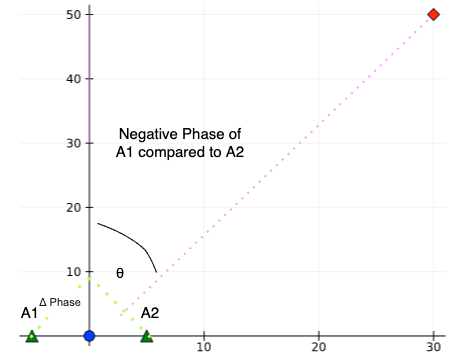
\includegraphics[width=.3\linewidth]{Images/diagrams/phase_negative.png}}\hfill
    \subfloat[No Phase]{\label{b}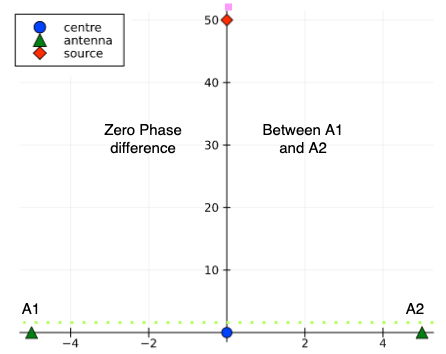
\includegraphics[width=.3\linewidth]{Images/diagrams/no_phase.png}}\hfill 
    \subfloat[Positive Phase]{\label{c}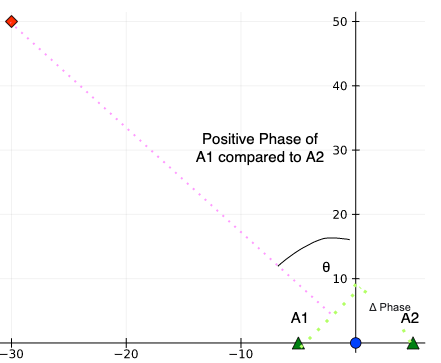
\includegraphics[width=.28\linewidth]{Images/diagrams/phase_positive.png}}
    \caption{Movement of the transmission source and resultant change in phase perceived at the antenna array}
    \label{fig:phase-change}
\end{figure}

As shown in Figure \ref{fig:phase-change}, movement of the transmission source \emph{should} cause a change in the phase difference (calculated as per section \ref{sec:Signal-Theory}). This test is conducted as the major testing portion of the project.

With the signal generator outputting the test transmission signal (Figure \ref{fig:function-gen}) and connected to an antenna, measurements of the phase will be taken. To do this, algorithm \ref{alg:loop} will be run, where the phase will be captured, a pause to move the transmission source, and then phase captured again. This testing was performed in a lab, with the cable between the transmitter and signal generator that was long enough to move from $-\frac{\pi}{4}$ to $\frac{\pi}{4}$. Reflections within the lab will have caused some minor interference, however, the dominant signal will still be the directly received signal. Great care is taken to measure the actual \gls{AoA}, as well as the distance moved of the transmission source to produce the table \ref{tab:phase-results} in Chapter \ref{ch:results}.

\begin{figure}[h]
  \vspace{0.2cm}
  \centering
  \captionsetup{type=figure}
  \begin{minipage}[5cm]{.7\linewidth}
    \begin{algorithm}[H]
      \caption{Loop for testing phase while moving transmission source.\label{alg:loop}}
      \DontPrintSemicolon
      \SetAlgoLined
      \BlankLine
          \Begin{
          \gls{sdr} \leftarrow \text{connection}\\
          \gls{sdr} \leftarrow \text{initialisation via init file}
          
          \While(){TRUE}{
            \For{\text{<0.1 second>}}{
                \text{Sample data at each Antenna: A1,A2} \\
                \text{Store sampled data to .iq files}} \\
            \\    
            \text{a1\_data, a2\_data} \leftarrow \text{Read data from files to array}  \\  
            \text{A1, A2} \leftarrow \text{fft(a1\_data), fft(a2\_data)}\\
            \\
            \\
            \text{maxsignal\_1} \leftarrow \text{Index of max magnitude in A1} \\
            \text{maxsignal\_2} \leftarrow \text{Index of max magnitude in A2} \\
            \\
            \text{phase\_1} \leftarrow \text{A1[maxsignal\_1]} \\
            \text{phase\_2} \leftarrow \text{A1[maxsignal\_2]} \\
            
            \While(){\text{Move transmitter to next location}}{
                \text{Wait}} \\
            \Return \text{phase\_1, phase\_2}}}
    \vspace{0.2cm}
    \end{algorithm}
  \end{minipage}
\end{figure}


* Note that phase\_1 and phase\_2 are complex phasors in the format $a \pm j b$
\subsection{Sample Length}
As can be seen in the pseudo-code provided in algorithm \ref{alg:loop}, data is captured for 0.1 of a second, and calculations are performed on this. It is assumed that given a continuous signal at a frequency of 150.5MHz, this will provide sufficient data points to perform the \gls{fft} on, and extract a meaningful phase from. However, given that the data may be noisy (from both reflections within the lab, and external \gls{em} waves of unknown sources), the following hypothesis is proposed: 

\emph{"It is true to say that doing one \gls{fft} on 1s of recorded data gives better accuracy than doing 100 \gls{fft}s on 0.01s recordings, and taking the average."}

To test this hypothesis, and determine the minimum duration of data capture on which phase extraction can be performed, data capture for varying lengths will be recorded and discussed with statistical analysis in Chapter \ref{ch:results}. 

\subsection{Averaging}
The final test for this project is that of averaging. Given that the recorded data may be noisy, averaging of the complex phasor may be necessary to determine an accurate \gls{AoA}.

If signal processing operations are linear, then it does not matter if averaging is done before or after the processing. However, in this case, the calculation of an \gls{AoA} is a non-linear function of phase, therfore there will be a difference, although it may not be significant unless the data is very noisy.

In order to test this, an analysis was be done on the phases collected during testing as described in \ref{sec:collection}. If averaging of the calculated \gls{AoA} is performed, a small bias may be introduced into the calculated results. Thus, the phase difference will instead be averaged, before \gls{AoA} calculations. 

For each iteration, without moving the signal source, the complex phasors phase\_1 and phase\_2 are returned. Letting:
\begin{equation*}
\begin{split}
    phase\_1 & = V1 \\
    phase\_2 & = V2 \\
\end{split}
\end{equation*}
then
\begin{equation*}
    Z = V1 * conj(V2)
 \end{equation*}  
will give the \gls{pd}. Running this for $x$ iterations, and then taking the average of $Z$ should produce clearer \gls{pd} results. This will be tested and verified. 

In addition, with a large number of phase data points, plotting of a histogram, calculation of the mean and standard deviation will be conducted. 

In order to validate that averaging of the results is necessary, one needs to prove the following:
If the standard deviation from one measurement is $s$, then averaging $N$ measurements reduces the standard deviation to $s \sqrt{N}$.


%---------------------------------
% Summary
%---------------------------------
\section{Summary}
This chapter thoroughly explored the approach and methodology of this project. By a top-down approach of a \gls{sdr} \gls{df} system, starting with a fundamental understanding of the signal processing theory, with respect to \gls{dsp}. Following this, a high-level overview of the hardware components that will be needed for a prototype project, discussing the design considerations and selection of the devices. The overview and considerations of the software needed to develop this project was discussed, and the considerations with respect to the goals of the project were taken into acccount. Finally, a testing procedure is presented. 
% ----------------------------------------------------
\ifstandalone
\bibliography{Bibliography/References}
\printnoidxglossary[type=\acronymtype, nonumberlist]
\fi
\end{document}
 % ----------------------------------------------------